%!TEX root = ../principal.tex
\setchapterimage[7.5cm]{figs/unidim/puente-tren}
\setchapterpreamble[u]{\margintoc}

\chapter{Elementos finitos en una dimensión}

\begin{kaobox}
	``No conocemos una millonésima parte del uno por ciento de nada”
	\begin{flushright}
		Thomas A. Edison
	\end{flushright}
\end{kaobox}

\section{Ejercicios resueltos}

\begin{example}
	Considere la barra de la fig. \ref{fig:unid}. El área transversal $A_e$ es de $7.75 \, \unit{cm^2}$ y el módulo de Young $E = 200 \, \unit{GPa}$. Si $q_1 = 0.5 \, \unit{mm}$ y $q_2 = 0.625 \, \unit{mm}$, determine:

\begin{enumerate}[noitemsep]
	\item La coordenada $\xi$ y el desplazamiento en el punto $P$;
	\item La deformación unitaria $\varepsilon$ y el esfuerzo $\sigma$;
	\item La matriz de rigidez del elemento;
	\item La energía de deformación unitaria del elemento.
\end{enumerate}

\begin{marginfigure}[-3cm]
	\centering
	\includestandalone[width=\textwidth]{figs/unidim/barra1}
	\caption{Elemento finito unidimensional.}
	\label{fig:unid}
\end{marginfigure}

\textit{Solución}:
\vspace{2mm}

\begin{enumerate}[label=\textbf{\arabic*}.]
	\item Coordenada $\xi$ y desplazamiento en $P$
	\begin{itemize}
		\item Coordenada $\xi$ del punto $P$:
		
		La coordenada $\xi$ se calcula con: $$\xi = \dfrac{2}{l_e} \left( x - x_1 \right) - 1$$
		
		para los datos del problema, resulta:
		
		$$\boxed{\xi_P = 0.364}$$
		
		\item Desplazamiento en el punto $P$:
		
		Se obtiene por interpolación de $q_1$ y $q_2$:
		
		$$
		\tilde{u}(\xi) = q_1 N1 + q_2 N_2 = q_1 \dfrac{1-\xi}{2} + q_2 \dfrac{1+\xi}{2} 
		$$
		
		$$
		u_P = q_1 \dfrac{1-\xi_P}{2} + q_2 \dfrac{1+\xi_P}{2}
		$$
		
		$$
		\boxed{u_P = 0.585 \, \unit{mm}}
		$$
	\end{itemize}

\item Deformación unitaria $\varepsilon$ y esfuerzo $\sigma$
\begin{itemize}
	\item Deformación unitaria
	
	\begin{equation}
		\varepsilon = \dfrac{du}{dx} = \dfrac{du}{d \xi} \dfrac{d \xi}{dx} = \left( -\dfrac{1}{2} q_1 + \dfrac{1}{2}q_2 \right) \dfrac{2}{l_e} = \dfrac{q_2 - q_1}{l_e}
		\label{eq:epsilon_tema2}
	\end{equation}
	
	$$
	\boxed{\varepsilon = \num{5.68e-4}}
	$$
	
	\item Esfuerzo
	$$
	\sigma = E \varepsilon
	$$
	
	$$
	\boxed{\sigma = 113.64 \, \unit{MPa}}
	$$
\end{itemize}

\item Matriz de rigidez del elemento:
		$$
\mathbf{k} = \dfrac{A_eE}{l_e} \left[ \begin{array}{rr}
	1 & -1 \\ -1 & 1
\end{array} \right]
$$

$$
\boxed{\mathbf{k} = \num{704.5e6} \left[ \begin{array}{rr}
		1 & -1 \\ -1 & 1
	\end{array} \right] \, \unit{N/m} }
$$

\item Energía de deformación unitaria del elemento:
$$
U = \dfrac{1}{2} \int_V \sigma^T \varepsilon dV = \dfrac{1}{2} \int_L \sigma^T \varepsilon A_e \, dx = \dfrac{1}{2} \sigma \varepsilon A_e L
$$

$$
\boxed{U = 11.01 \, \unit{J}}
$$
\end{enumerate}
\end{example}

Esta es una ecuación fuera de ejemplos, para ver qué enumeración tiene asignada:
\begin{equation}
	y=x
\end{equation}

\begin{example}
	Calcule el desplazamiento en el extremo libre de la barra de la figura utilizando elementos finitos lineales. $E = 25 \unit{GPa}$.
	\begin{figure}[H]
		\centering
		\includestandalone[width=.7\textwidth]{figs/unidim/barra2}
	\end{figure}
\textit{Solución}:
\vspace{2mm}

Fórmulas para las matrices de rigidez y vectores de carga:
\begin{itemize}
    \item Matriz de rigidez: $\mathbf{k} = \dfrac{A_eE_e}{l_e} \left[\begin{array}{rr}
		1 & -1 \\ -1 & 1
	\end{array}\right]$
	\item Vector de cargas: $\mathbf{P} = \dfrac{pl_e}{2} \begin{bmatrix}
		1 \\ 1
	\end{bmatrix}$
\end{itemize}
Se analiza a continuación por número de elementos finitos:
\begin{itemize}
	\item \textbf{1 Elemento finito}
	
	\begin{marginfigure}[-1cm]
		\centering
		\begin{tikzpicture}[scale=1.5]
			\draw[pattern=north west lines, pattern color=blue] (-.15, -.3) rectangle (0, .3);
			\draw[fill=blue!10] (0,-.2) -- (0, .2) -- (2, .1) -- (2, -.1) -- cycle;
			\draw[|-|] (0, -.4) -- (2, -.4) node[pos=.5, below] {$2\unit{m}$};
			
			% Carga distribuida
			\foreach \x in {0.05, .45, .85, 1.25, 1.65}{
				\draw[-latex, red, thick] (\x, 0) -- (\x + .3, 0);}
			\draw[-latex, very thick] (2, 0) -- (2.4, 0) node[pos=.8, above]{$10\unit{kN}$};
			
			% 1EF
			\draw[dashed, thick] (0, -.15) rectangle (2, .15);
			
			\draw[very thick] (0, -1) -- (2, -1);
			\foreach \i in {0, 2}{
				\node[draw, circle, fill=black] at (\i, -1) {};
			}
			\draw[-latex, red, very thick] (-.5, -1) -- (-.1, -1) node[pos=.5, above]{$2$};
			\draw[red, very thick] (-.4, -1.05) -- (-.3, -.95);  %tacha
			\draw[-latex, red, very thick] (2.1, -1) -- (2.4, -1) node[pos=.5, above]{$1$};
		\end{tikzpicture}
	\caption*{\centering 1 elemento finito}
	\end{marginfigure}

Valores:
	$L_1 = 2 \unit{m}; \quad A_1 = 20\times 30 \unit{cm^2}; \quad p_1 = p(1) = 3 \unit{kN/m}$
	
Matriz de rigidez y vector de cargas:
	$$\mathbf{k}_1 = \num{750e6} \begin{blockarray}{ccc}
		\color{red} 2 & \color{red} 1\\
		\begin{block}{[rr]c}
			1 & -1 & \color{red} 2\\
			-1 & 1 & \color{red} 1\\
		\end{block}
	\end{blockarray}\ \unit{[N/m]}$$ $$\mathbf{P} = \num{3e3}  \begin{blockarray}{cc}
	\begin{block}{[r]c}
		1 & \color{red} 2 \\ 1 & \color{red} 1\\
	\end{block}
\end{blockarray} [\unit{N}]$$

Ensamble:
$$ S = \num{750e6} \ \unit{N/m}; \quad F = \num{3e3} \ \unit{N} $$
Resultado: $\delta = S^{-1}F$
$$
\boxed{\delta = \num{4e-6} \unit{m}}
$$
	
\item \textbf{2 Elementos finitos}
\begin{marginfigure}[-1cm]
	\centering
	\begin{tikzpicture}[scale=1.5]
		\draw[pattern=north west lines, pattern color=blue] (-.15, -.3) rectangle (0, .3);
		\draw[fill=blue!10] (0,-.2) -- (0, .2) -- (2, .1) -- (2, -.1) -- cycle;
		\draw[|-|] (0, -.4) -- (1, -.4) node[pos=.5, below] {$1\unit{m}$};
		\draw[-|] (1, -.4) -- (2, -.4) node[pos=.5, below] {$1\unit{m}$};
		
		% Carga distribuida
		\foreach \x in {0.05, .45, .85, 1.25, 1.65}{
			\draw[-latex, red, thick] (\x, 0) -- (\x + .3, 0);}
		\draw[-latex, very thick] (2, 0) -- (2.4, 0) node[pos=.8, above]{$10\unit{kN}$};
		
		% 2EF
		\draw[dashed, thick] (0, -.175) rectangle (1, .175);
		\draw[dashed, thick] (1, -.125) rectangle (2, .125);
		
		\draw[very thick] (0, -1) -- (2, -1);
		\foreach \i in {0, 1, 2}{
			\node[draw,circle, fill=black] at (\i, -1) {};
		}
		\draw[-latex, red, very thick] (-.5, -1) -- (-.1, -1) node[pos=.5, above]{$3$};
		\draw[red, very thick] (-.4, -1.05) -- (-.3, -.95);  % tacha
		\draw[-latex, red, very thick] (1.1, -1) -- (1.4, -1) node[pos=.5, above]{$1$};
		\draw[-latex, red, very thick] (2.1, -1) -- (2.4, -1) node[pos=.5, above]{$2$};
	\end{tikzpicture}
\caption*{\centering 2 elementos finitos}
\end{marginfigure}

\begin{itemize}
	\item Elemento 1
	
	$L_1 = 1 \unit{m}; \quad A_1 = 20\times 35 \unit{cm^2}; \quad p_1 = p(0.5) = 3.75 \unit{kN/m}$
	
	Matriz de rigidez y vector de cargas:
	$$
	\mathbf{k}_1 = \num{1750e6} \begin{blockarray}{ccc}
		\color{red} 3 & \color{red} 1\\
		\begin{block}{[rr]c}
			1 & -1 & \color{red} 3\\
			-1 & 1 & \color{red} 1\\
		\end{block}
	\end{blockarray} \ \unit{[N/m]}
	$$
	
	$$\mathbf{P}_1 = 1875  \begin{blockarray}{cc}
		\begin{block}{[r]c}
			1 & \color{red} 3 \\ 1 & \color{red} 1\\
		\end{block}
	\end{blockarray} [\unit{N}]$$
	
	\item Elemento 2
	
	$L_2 = 2 \unit{m}; \quad A_2 = 20\times 25 \unit{cm^2}; \quad p_2 = p(1.5) = 1.75 \unit{kN/m}$
	
		$$
	\mathbf{k}_2 = \num{1250e6} \begin{blockarray}{ccc}
		\color{red} 1 & \color{red} 2\\
		\begin{block}{[rr]c}
			1 & -1 & \color{red} 1\\
			-1 & 1 & \color{red} 2\\
		\end{block}
	\end{blockarray} \ \unit{[N/m]}
	$$
	
	$$\mathbf{P}_2 = 875  \begin{blockarray}{cc}
		\begin{block}{[r]c}
			1 & \color{red} 1 \\ 1 & \color{red} 2\\
		\end{block}
	\end{blockarray} [\unit{N}]$$

\item Ensamble

$$
\mathbf{S} = \num{1e6} \left[\begin{array}{rr}
	3000 & -1250 \\ -1250 & 1250
\end{array}\right] \ [\unit{N/m}]
$$

$$
\mathbf{F} = \begin{bmatrix}
	2750 \\ 875
\end{bmatrix} \ \unit{N}
$$

\item Resultado
$$
\mathbf{D} = \mathbf{S}^{-1} \mathbf{P} = \begin{bmatrix}
	2.07 \\ 2.77
\end{bmatrix} \num{1e-6}
$$

$$
\boxed{\delta = \num{2.77e-6} \unit{m}}
$$
\end{itemize}
\end{itemize}
\end{example}
Otro ejemplo.
\begin{example}
	La barra circular tiene un radio variable $r=r_0 e^{ax}$ y está fabricada de un material con módulo de elasticidad $E$. Determine el desplazamiento del extremo libre cuando se somete a la fuerza axial $P$. Resolver por los siguientes métodos y calcular en todos los caso el campo de tensiones correspondiente:
	\begin{enumerate}[noitemsep]
		\item Rayleigh-Ritz;
		\item Galerkin;
		\item Utilizando dos elementos finitos lineales.
		\item Adoptar los valores siguientes y comparar los resultados:
		\begin{equation}
			\begin{split}
				&a = 0.2 \, \unit{m^{-1}}; \ E = 25\, \unit{GPa}; \ L = 2 \, \unit{m}; \\ &P = 100 \, \unit{kN}; \ r_0 = 0.10\, \unit{m}
			\end{split}
			\label{eq:datos}
		\end{equation}
	\end{enumerate}
	
	\begin{marginfigure}[-5cm]
		\centering
		\def\L{6}
		\def\r0{.4}
		\def\a{-.2}
		\begin{tikzpicture}[scale=.7]
			\draw[thick, domain=-\L.:0, variable=\x, yscale=1] plot({\x}, {\r0*exp(\a*\x)});
			\draw[thick, domain=-\L:0, variable=\x, yscale=1] plot({\x}, {-\r0*exp(\a*\x)});
			\draw[thick] (0,-\r0) -- (0, \r0);
			
			% Cotas
			\draw[|-|] (-\L, -1.6) -- (0, -1.6) node[pos=.5, above]{$L$};
			\draw[] (-\L, 0) -- (0, 0);
			\node at (.3, .3) {$r_0$};
			\draw[-latex, thick] (-\L*.75, 0) -- (-\L*.75, 1) node[pos=.5, right]{$r$};
			%\draw[-latex] (1.6, 0) -- (2.3, 0) node[below]{$x$};
			
			
			% Fuerza
			\draw[very thick, red, -latex] (.1, 0) -- (1, 0) node[below]{$P$};
			
			% Apoyos
			\draw[pattern=north west lines] (-\L - .5, -1.9) rectangle (-\L, 1.9);
		\end{tikzpicture}
		\caption{Barra a tracción de sección variable}
		\label{fig:tema3}
	\end{marginfigure}

\textit{Solución}
\vspace{2mm}

	Se observa que el origen de coordenadas debe estar en el extremo derecho de la barra, con lo cual $$r(0) = r_0$$ el valor del radio en el empotramiento será: $r(-L) = r_0 e^{-aL}$, ahora bien, según el gráfico, el área a la izquierda es mayor que a la derecha, es decir $r(-L) > r(0)$, de donde $e^{-aL} > 1$, por lo que $a < 0$, para poner en evidencia este hecho, adoptamos $a > 0$, y escribimos la ecuación:
	
	\begin{equation}
		r = r_0 e^{-ax} \qquad \mbox{con } a, r_0 > 0
	\end{equation}
	
	Estas observaciones se ilustran en la fig. \ref{fig:tema3a}.
	
	\begin{figure}[H]
		\centering
		\def\L{6}
		\def\r0{.4}
		\def\a{-.2}
		\begin{tikzpicture}[scale=.9]
			\draw[thick, domain=-\L.:0, variable=\x, yscale=1] plot({\x}, {\r0*exp(\a*\x)});
			\draw[thick, domain=-\L:0, variable=\x, yscale=1] plot({\x}, {-\r0*exp(\a*\x)});
			\draw[thick] (0,-\r0) -- (0, \r0);
			
			% Cotas
			\draw[-|, thin] (-\L, -1.6) -- (0, -1.6) node[pos=.5, above]{$L$};
			\draw[] (-\L, 0) -- (0, 0);
			\node at (.3, .3) {$r_0$};
			\draw[-latex, thick] (-\L*.75, 0) -- (-\L*.75, 1) node[pos=.4, right]{$r=r_0e^{-ax}$};
			\draw[-latex] (1.6, 0) -- (2.3, 0) node[below]{$x$};
			\draw[-latex] (0,0) -- (0, 1.5) node[right]{$y$};
			\draw[fill] (0,0) circle (2pt);
			\node at (-\L+.5, .6) {$r_0e^{aL}$};
			\draw[latex-] (-\L, 1.5) -- (-\L*.85, 1.5) node[pos=.8, above]{$x=-L$};
			
			% Fuerza
			\draw[very thick, color=tt5, -latex] (.1, 0) -- (1, 0) node[right]{$P$};
			
			% Apoyos
			\draw[pattern=north west lines] (-\L - .5, -1.9) rectangle (-\L, 1.9);
		\end{tikzpicture}
		\caption{Sistema de coordenadas}
		\label{fig:tema3a}
	\end{figure}

\begin{enumerate}[label=\textbf{\arabic*}.]
	\item \textbf{Método de Rayleigh-Ritz}
	
	Se utiliza un polinomio de $2^o$ grado como función aproximadora:
	\begin{equation}
		\tilde{u}(x) = a_0 + a_1 x + a_2 x^2
		\label{eq:u}
	\end{equation}
	
	La única condición de frontera esencial es:
	\begin{equation}
		\begin{split}
			u(-L) &= 0 \\
			a_0 - a_1L + a_2 L^2 = 0 &\implies a_2 = \dfrac{a_1L - a_0}{L^2}
		\end{split}
		\label{eq:esencial}
	\end{equation}
	
	Las condiciones de frontera naturales están implícitas en el método.
	
	Llevando \eqref{eq:esencial} en \eqref{eq:u}:
	\begin{equation}
		\tilde{u}(x) = a_{0} + a_1 x + \dfrac{a_1L - a_0}{L^2} x^{2}
		\label{eq:u2}
	\end{equation}
	
	su derivada es:
	\begin{equation}
		\dfrac{d\tilde{u}}{dx} = a_1 + \dfrac{2}{L^2} \left(a_1L - a_0\right) x
		\label{eq:du}
	\end{equation}
	La energía potencial total, en este caso, es:
	$$
	\Pi = \dfrac{1}{2} \int_{-L}^0 EA \left( \dfrac{du}{dx} \right)^2 \, dx - u(0) P
	$$
	
	haciendo las substituciones pertinentes e integrando, se obtiene:
	\begin{equation}
		\begin{split}
			\Pi =& \dfrac{\pi Er_0^2}{4a^3L^4} \left( L^{4} a^{2} a_{1}^{2} e^{2 L a} - L^{4} a^{2} a_{1}^{2} - 4 L^{3} a^{2} a_{0} a_{1} e^{2 L a} \right.\\[1mm] & - 2 L^{3} a a_{1}^{2} e^{2 L a} - 2 L^{3} a a_{1}^{2} + 4 L^{2} a^{2} a_{0}^{2} e^{2 L a} + 6 L^{2} a a_{0} a_{1} e^{2 L a} \\[1mm] & + 2 L^{2} a a_{0} a_{1} + 2 L^{2} a_{1}^{2} e^{2 L a} - 2 L^{2} a_{1}^{2} - 4 L a a_{0}^{2} e^{2 L a} \\[1mm] & \left. - 4 L a_{0} a_{1} e^{2 L a} + 4 L a_{0} a_{1} + 2 a_{0}^{2} e^{2 L a} - 2 a_{0}^{2} \right) - a_0P
		\end{split}
	\end{equation}
	
	La energía potencial total debe ser mínima, es decir: $\dfrac{\partial \Pi}{\partial a_i} = 0$ 
	
	\begin{equation}
		\begin{split}
			\dfrac{\partial \Pi}{\partial a_0} =& \, 4a_{0} \left(2 L^{2} a^{2} e^{2 L a} - 2 L a e^{2 L a} + e^{2 L a} - 1 \right) + \\
			& 2a_{1}L \left(- 2 L^{2} a^{2} e^{2 L a} + 3 L a e^{2 L a} + 2 L a - 2 e^{2 L a} + 2 \right) \\ & - \dfrac{4a^3L^4P}{\pi E r_0^2} = 0
		\end{split}
		\label{eq:dPi0}
	\end{equation}
	
	\begin{equation}
		\begin{split}
			\dfrac{\partial \Pi}{\partial a_1} = &
			a_{0} \left(- 4 L^{2} a^{2} e^{2 L a} + 6 L a e^{2 L a} + 2 L a - 4 e^{2 L a} + 4 \right) + \\ & a_{1}L \left(2 L^{2} a^{2} e^{2 L a} - 2 L^{2} a^{2} - 4 L a e^{2 L a} - 4 L a + 4 e^{2 L a} - 4 \right) = 0
		\end{split}
		\label{eq:dPi1}
	\end{equation}
	
	de \eqref{eq:dPi0} y \eqref{eq:dPi1}:
	
\begin{equation}
	\begin{cases}
		a_0 =& \dfrac{2 L^{2} P a \left(- L^{2} a^{2} e^{2 L a} + L^{2} a^{2} + 2 L a e^{2 L a} + 2 L a - 2 e^{2 L a} + 2\right)}{\pi E r_{0}^{2} \left(4 L^{2} a^{2} e^{2 L a} - e^{4 L a} + 2 e^{2 L a} - 1\right)} \\[5mm]
		a_1 =& \dfrac{2 L P a \left(- 2 L^{2} a^{2} e^{2 L a} + 3 L a e^{2 L a} + L a - 2 e^{2 L a} + 2\right)}{\pi E r_{0}^{2} \left(4 L^{2} a^{2} e^{2 L a} - e^{4 L a} + 2 e^{2 L a} - 1\right)}
	\end{cases}
	\label{eq:constantes}
\end{equation}
	
	El campo de desplazamientos pedido se obtiene sustituyendo las constantes \eqref{eq:constantes} en \eqref{eq:u2}.
	
	En el extremo libre:
	
	\begin{equation}
		\boxed{\tilde{u}(0) = a_0}
	\end{equation}
	
	con $a_0$ dado en \eqref{eq:constantes}.
	
	Con los datos del problema se obtiene (en $\unit{mm}$):
	
	\begin{equation}
		\tilde{u}(x) = 0.017 x^2 + 0.122x + 0.175
	\end{equation}
	
	En el extremo libre:
	
	\begin{equation}
		\tilde{u}(0) = 0.175 \, \unit{mm}
		\label{eq:delta}
	\end{equation}
	
	\textbf{Campo de tensiones}
	
	Se obtiene de:
	\begin{equation}
		\sigma = E \dfrac{du}{dx}
		\label{eq:sigma}
	\end{equation}
	
	es decir, llevando \eqref{eq:constantes} en \eqref{eq:du} y luego en \eqref{eq:sigma}.
	
	Con los datos de \eqref{eq:datos}:
	
	\begin{equation}
		\sigma = 0.849 x + 3.039 \quad [\unit{MPa}]
	\end{equation}
	
	\item \textbf{Método de Galerkin}
	
	Reordenando términos en \eqref{eq:u2} se tiene:
	
	\begin{equation*}
		\tilde{u}(x) = a_{0} \left(1 - \frac{x^{2}}{L^{2}}\right) + a_1 x \left(1 + \frac{x}{L}\right) = a_0 \phi_1(x) + a_1 \phi_2(x)
	\end{equation*}

de donde las funciones base son:
\begin{align}
	\phi_1(x) &= 1 - \dfrac{x^2}{L^2}
	\label{eq:phi1} \\
	\phi_2(x) &= x \left( 1 + \dfrac{x}{L} \right)
	\label{eq:phi2}
\end{align}
	La ecuación diferencial del problema es:
	\begin{equation}
		\dfrac{d}{dx} \left(EA \dfrac{du}{dx}\right) + p(x) = 0
	\end{equation}
	
	en este caso: $p(x) = 0$.
	
	Imponemos la condición de ortogonalidad entre las funciones $\phi_i$ y el residual:
	\begin{equation}
		\int_L \phi_i(x) \dfrac{d}{dx} \left(EA \dfrac{d\tilde{u}}{dx}\right) \, dx = 0
	\end{equation}
	
	integrando por partes:
	$$\left[EA \dfrac{d\tilde{u}}{dx} \phi_i\right]_{-L}^0 - \int_L EA \dfrac{d\tilde{u}}{dx} \dfrac{d \phi_i}{dx} \, dx = 0$$
	
	$$\left.EA \dfrac{d\tilde{u}}{dx} \phi_i\right|_{x=0} - \left.EA \dfrac{d\tilde{u}}{dx} \phi_i\right|_{x=-L} - \int_L EA \dfrac{d\tilde{u}}{dx} \dfrac{d \phi_i}{dx} \, dx = 0$$
	
	como:
	$$
	\begin{cases}
		\phi_i(-L) = 0 & \mbox{condición de frontera de Dirichlet} \\[4mm]
		\left. EA \dfrac{d \tilde{u}}{dx}\right|_{x=0} = P & \mbox{condición de frontera de Neumann}
	\end{cases}
	$$
	se tiene:
	
	\begin{equation}
		\int_L EA \dfrac{d\tilde{u}}{dx} \dfrac{d \phi_i}{dx} \, dx = P \phi_i(0)
		\label{eq:integral}
	\end{equation}
	
	que es la ecuación del trabajo virtual.
	
	Integrando con $\phi_1(x)$ dado en \eqref{eq:phi1} se obtiene la ecuación \eqref{eq:dPi0} e integrando con $\phi_2(x)$ dado en \eqref{eq:phi2} se obtiene \eqref{eq:dPi1}, es decir, las soluciones son idénticas al método de Rayleigh-Ritz.

\item \textbf{Método de elementos finitos}.

\begin{marginfigure}[-1cm]
\centering
\begin{tikzpicture}[scale=1.9]
	\draw[fill=black!30] (0,-.05) rectangle (2, .05);
	\draw[->, thin] (0, 0) -- (2.5, 0) node[below]{$x$};
	\draw[fill=black] (0,0) circle (1pt) node[left]{$1$};
	\draw[fill=black] (1,0) circle (1pt) node[below right]{$2$};
	\draw[fill=black] (2,0) circle (1pt) node[below right]{$3$};
	
	\draw[->, very thick, tt5] (0, .2) -- (.3, .2) node[pos=.5, above left]{$3$};
	\draw[very thick, tt5] (0.12, .15) -- (0.18, .25);
	\draw[->, very thick, tt5] (1, .2) -- (1.3, .2) node[pos=.5, above]{$1$};
	\draw[->, very thick, tt5] (2, .2) -- (2.3, .2) node[pos=.5, above]{$2$};
\end{tikzpicture}
\caption{Modelo}
\end{marginfigure}

\begin{itemize}
\item \textbf{Elemento 1}

Los valores medios son:

$r(-3L/4) = r_0 \exp \left(\frac{3aL}{4}\right); \ A_1 = \pi r_0^2 \exp \left(\frac{3aL}{2}\right)$

La longitud del elemento es: $l_e = \dfrac{L}{2}$.

El vector de cargas no tiene componentes en los grados de libertad. La matriz de rigidez es:

$$\mathbf{k}_1 = \dfrac{2\pi r_0^2 E \exp \left(\frac{3aL}{2}\right)}{L} \begin{blockarray}{ccc}
	\color{red} 3 & \color{red} 1\\
	\begin{block}{[rr]c}
		1 & -1 & \color{red} 3\\
		-1 & 1 & \color{red} 1\\
	\end{block}
\end{blockarray}$$

\item \textbf{Elemento 2}

$ r(-L/4) = r_0 \exp \left(\frac{aL}{4}\right); \ A_2 = \pi r_0^2 \exp \left(\frac{aL}{2}\right); \, l_e = \dfrac{L}{2} $

Matriz de rigidez:

$$\mathbf{k}_2 = \dfrac{2\pi r_0^2 E \exp \left(\frac{aL}{2}\right)}{L} \begin{blockarray}{ccc}
	\color{red} 1 & \color{red} 2\\
	\begin{block}{[rr]c}
		1 & -1 & \color{red} 1\\
		-1 & 1 & \color{red} 2\\
	\end{block}
\end{blockarray}$$

Vector de cargas:
$$
\mathbf{P}_2 = \begin{bmatrix}
	0 \\ P
\end{bmatrix}
$$

\item \textbf{Ensamble}

Matriz de rigidez y vector de cargas en los grados de libertad:
$$\mathbf{S} = \dfrac{2\pi r_0^2 E \exp \left( \frac{aL}{2} \right)}{L} \left[ \begin{array}{cc}
	\exp \left(aL\right) + 1 & -1 \\[4mm] -1 & 1
\end{array} \right]; \quad \mathbf{F} = \begin{bmatrix} 0 \\ P \end{bmatrix}$$

\item \textbf{Soluciones}

\begin{equation}
	\mathbf{D} = \mathbf{S}^{-1} \mathbf{F} = \dfrac{PLe^{-\frac{3aL}{2}}}{2\pi E r_0^2} \left[\begin{matrix} 1\\[4mm] 1 + e^{aL}\end{matrix}\right]
	\label{eq:D}
\end{equation}

En el extremo libre:
\begin{equation}
	\boxed{\delta_2 = \dfrac{PLe^{-\frac{3aL}{2}}}{2\pi E r_0^2} \left( 1 + e^{aL} \right)}
\end{equation}

Incorporando los valores dados en \eqref{eq:datos}, se tiene:
$$
\mathbf{D} = \begin{bmatrix}
	0.070 \\[1mm] 0.174
\end{bmatrix} \ \unit{mm}
$$

con lo cual:
\begin{equation}
	\delta_2 = 0.174 \, \unit{mm}
	\label{eq:delta2}
\end{equation} observe la cercanía de este valor  con \eqref{eq:delta}.

\item \textbf{Tensiones}

Se vió en \eqref{eq:epsilon_tema2} que:
$$
\varepsilon = \dfrac{q_2 - q_1}{l_e}
$$

entonces:
\begin{equation}
	\sigma = \dfrac{q_2 - q_1}{l_e}E
	\label{eq:sigma2}
\end{equation}

Las valores $q_1$ y $q_2$ se obtienen observando \eqref{eq:D}, por lo tanto, aplicando \eqref{eq:sigma2} para cada elemento se tiene:
\begin{itemize}
	\item Elemento 1
	$$
	\sigma_1 = \dfrac{PLe^{-\frac{3aL}{2}}}{2\pi r_0^2}
	$$
	
	\item Elemento 2
	$$
	\sigma_2 = \dfrac{PLe^{-\frac{aL}{2}}}{2\pi r_0^2}
	$$
\end{itemize}

Para los datos de \eqref{eq:datos}: $\sigma_1 = 1.75 \, \unit{MPa}; \quad \sigma_2 = 2.61 \, \unit{MPa}$.

\item \textbf{Solución exacta}

Considerando la fig. \ref{fig:seccionT3}, la fuerza normal en una sección genérica de la barra es:

\begin{marginfigure}[-1cm]
	\centering
	\def\L{6}
	\def\r0{.4}
	\def\a{-.2}
	\begin{tikzpicture}[scale=.75]
		\draw[thick, domain=-\L.:-\L/2, variable=\x, yscale=1] plot({\x}, {\r0*exp(\a*\x)});
		\draw[thick, domain=-\L:-\L/2, variable=\x, yscale=1] plot({\x}, {-\r0*exp(\a*\x)});
		\draw[thick] (-\L/2,-1) -- (-\L/2, 1);
		
		% Cotas
		\draw[|-|] (-\L, -1.6) -- (-\L/2, -1.6) node[pos=.5, above]{$L-x$};
		\draw[] (-\L, 0) -- (-\L/2, 0);
		\draw[-latex, thick] (-\L*.75, 0) -- (-\L*.75, 1) node[pos=.5, right]{$r$};
		\draw[latex-] (-\L, 1.5) -- (-\L*.85, 1.5) node[pos=.8, above]{$x=-L$};
		\draw[latex-] (-\L/2, .9) -- (-\L*.35, .9) node[pos=.8, above]{$x$};
		
		
		% Fuerzas
		\draw[very thick, blue, -latex] (-\L/2, 0) -- (-\L/3, 0) node[below, pos=1.2]{$N=EA \dfrac{du}{dx}$};
		\draw[very thick, blue, -latex] (-\L-.55, 0) -- (-\L-1.5, 0) node[above, pos=.75]{$R = P$};
		
		% Apoyos
		\draw[pattern=north west lines] (-\L - .5, -1.9) rectangle (-\L, 1.9);
	\end{tikzpicture}
	\caption{Diagrama de cuerpo libre}
	\label{fig:seccionT3}
\end{marginfigure}

\begin{equation}
	N(x) = EA \dfrac{du}{dx} = P
\end{equation}

integrando de $-L$ a $x$:

\begin{equation}
	\int_{-L}^{x} du = \int_{-L}^{x} \dfrac{P}{EA} \, dx
\end{equation}
$$
u(x) - \cancelto{0}{u(-L)} \; \; \; = \dfrac{P e^{- 2 L a}}{2 \pi E a r_{0}^{2}} \left[e^{2a\left(L + x\right)} - 1\right]
$$
\begin{equation}
	\boxed{u(x) = \dfrac{P e^{- 2aL}}{2 \pi E a r_{0}^{2}} \left[e^{2a\left(L + x\right)} - 1 \right]
		\label{eq:exacto}}
\end{equation}
Las tensiones son:
\begin{equation}
	\sigma = E \dfrac{du}{dx} = \dfrac{Pe^{2ax}}{\pi r_0^2}
\end{equation}
Con los datos de \eqref{eq:datos}:
\begin{equation}
	u(x) = 0.318 e^{0.4x} - 0.143 \quad \unit{[mm]}
\end{equation}
\begin{equation}
	\sigma = 3.18 e^{0.4x} \quad [\unit{MPa}]
\end{equation}
En el extremo derecho:
\begin{equation}
	u(0) = 0.174 \, \unit{mm}
\end{equation}
comparar con \eqref{eq:delta} y \eqref{eq:delta2}.

\item \textbf{Gráficos comparativos}
\begin{figure}[H]
	\centering
	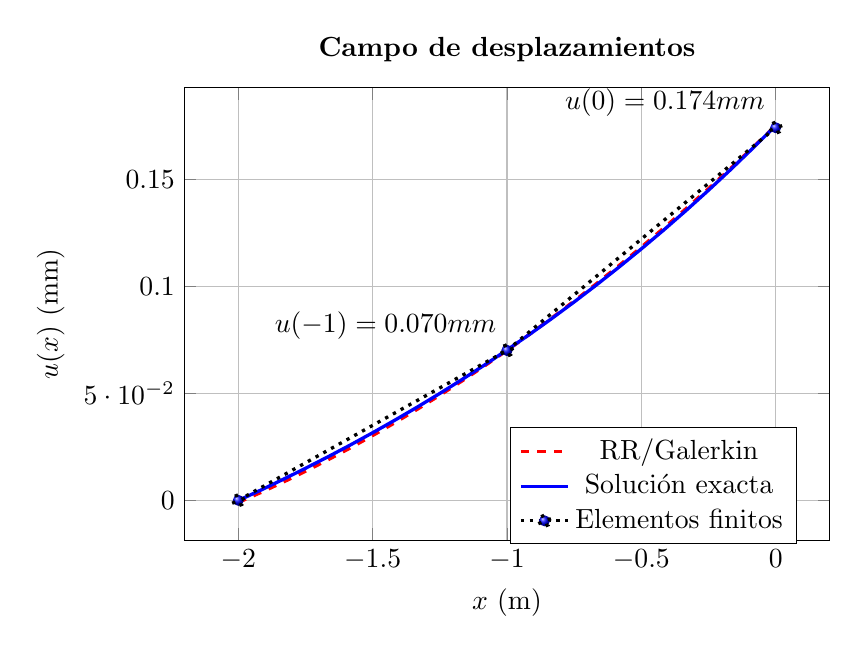
\begin{tikzpicture}
		\begin{axis}[scale=1.3, domain=-2:0, xlabel=$x$ (m), ylabel=$u(x)$ (mm), grid=both, title=\textbf{Campo de desplazamientos}, legend style={at={(.95, .25)}}, width=.65\textwidth, height=6cm, xtick distance=.5]
			\addplot[color=red, very thick, dashed] {0.017*x*x + 0.122*x + 0.175};
			\addlegendentry{RR/Galerkin}
			\addplot[color=blue, very thick] {0.318*exp(0.4*x) - 0.143};
			\addlegendentry{Solución exacta}
			\addplot[very thick, dotted, mark=ball] coordinates {(-2,0) (-1, 0.07)} node[above left]{$u(-1) = 0.070 \unit{mm}$};
			\addplot[very thick, dotted, mark=ball] coordinates {(-1, 0.07) (0, 0.174)} node[above left]{$u(0) = 0.174 \unit{mm}$};
			\addlegendentry{Elementos finitos};
		\end{axis}
	\end{tikzpicture}
	\caption{Comparación de resultados de desplazamientos}
\end{figure}

\begin{figure}[H]
	\centering
	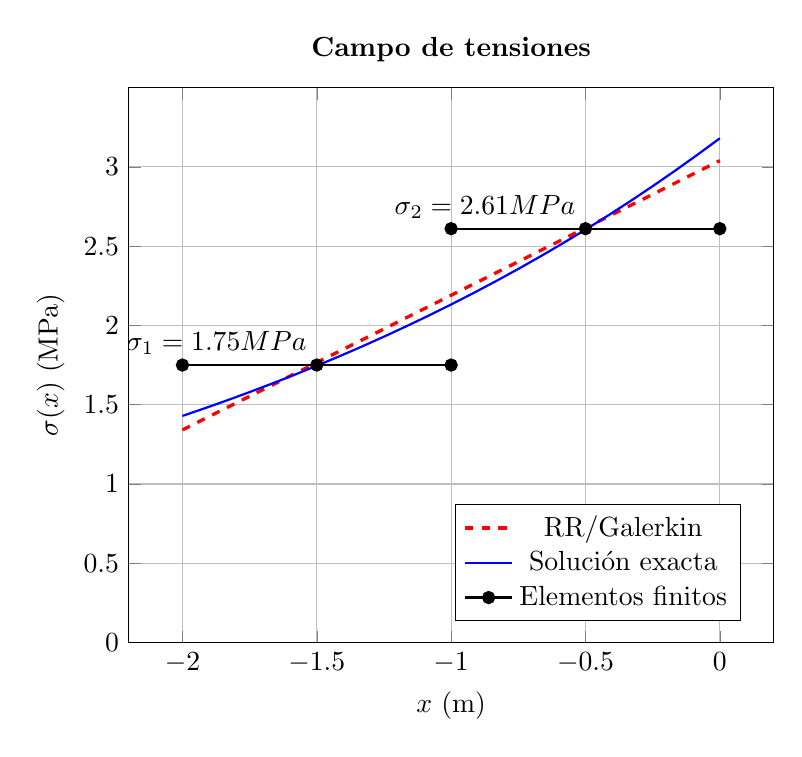
\begin{tikzpicture}
		\begin{axis}[scale=1.3, domain=-2:0, xlabel=$x$ (m), ylabel=$\sigma(x)$ (\unit{MPa}), grid=both, title=\textbf{Campo de tensiones}, legend style={at={(.95, .25)}}, width=.65\textwidth, height=7cm, xtick distance=.5, ymin=0]
			\addplot[color=red, very thick, dashed] {0.849*x + 3.039};
			\addlegendentry{RR/Galerkin}
			\addplot[color=blue, thick] {3.18*exp(0.4*x)};
			\addlegendentry{Solución exacta}
			\addplot[domain=-2:-1, thick, mark=*, samples=3] {1.75} node[above left, pos=.5]{$\sigma_1 = 1.75 \unit{MPa}$};
			\addplot[domain=-1:0, thick, mark=*, samples=3] {2.61} node[above left, pos=.5]{$\sigma_2 = 2.61 \unit{MPa}$};
			\addlegendentry{Elementos finitos};
		\end{axis}
	\end{tikzpicture}
	\caption{Comparación de resultados de tensiones}
\end{figure}
\end{itemize}
\end{enumerate}
\end{example}
